\section{Experiments}\label{sec:experiments}

The \DIFdelbegin \DIFdel{proposed multi-user preference learning model }\DIFdelend \DIFaddbegin \DIFadd{performance of the new muti-task preference model with BALD (MT-B)
}\DIFaddend is evaluated in a series of experiments with simulated \DIFaddbegin \DIFadd{and real-world }\DIFaddend data.
We \DIFaddbegin \DIFadd{compare MT-B with two versions of the proposed muti-task model
based on maximum entropy sampling (MT-E) and a random approach (MT-R) for
active learning. We also evaluate the performance of a single task method
with BALD (ST-B), maximum entropy sampling (ST-E) and a random approach (ST-R).
ST fits a different GP classifier to the item preferences of each user.
Finally, the last benchmark method is the muti-task method of }\cite{birlutiu2009} \DIFadd{using
BALD (MB-B), maximum entropy sampling (MB-E) and the random approach (MB-R).
A description of the implementation of MB can be found in the supplementary material.
}

\subsection{\DIFadd{Experiments with Simulated Data}}

\DIFadd{For the experiments with simulated data
we }\DIFaddend generate a total of \DIFdelbegin \DIFdel{$I=20$ }\DIFdelend \DIFaddbegin \DIFadd{$I=15$ }\DIFaddend synthetic items with features given by 2-dimensional vectors,
where the $i$-th item satisfies
\DIFdelbegin \DIFdel{$\x_i=(x_{i1},x_{i2})$ with $x_{i1},x_{i2} \sim U[-5, 5]$}\DIFdelend \DIFaddbegin \DIFadd{$\mathbf{x}_i=(x_{i1},x_{i2})$ and $x_{i1}$ and $x_{i2}$ follow a uniform distribution with zero mean and unit standard deviation}\DIFaddend .
The preferences of each user are \DIFdelbegin \DIFdel{given
}\DIFdelend \DIFaddbegin \DIFadd{generated
}\DIFaddend by a linear combination of $D=5$ latent functions $h_1,\ldots,h_5$. These functions are sampled from a \DIFdelbegin \DIFdel{GP
}\DIFdelend \DIFaddbegin \DIFadd{Gaussian process
}\DIFaddend with zero mean and preference \DIFdelbegin \DIFdel{covariance function generated }\DIFdelend \DIFaddbegin \DIFadd{kernel given }\DIFaddend by a squared exponential kernel with unit length-scale.
The preferences for the $u$-th user are obtained according to 
\DIFdelbegin \DIFdel{$g_u(\x, \x') = \text{sign}\{ \sum_{d=1}^5 w_{ud} h_d(\x, \x') + \epsilon_{\x,\x'} \}$}\DIFdelend \DIFaddbegin \DIFadd{$g_u(\mathbf{x}_i, \mathbf{x}_j) = \text{sign}\{ \sum_{d=1}^5 w_{ud} h_d(\mathbf{x}_i, \mathbf{x}_j) + \epsilon_{ij} \}$}\DIFaddend ,
where $w_{u1},\ldots,w_{u5}$ and \DIFdelbegin \DIFdel{$\epsilon_{\x, \x'}$ }\DIFdelend \DIFaddbegin \DIFadd{$\epsilon_{ij}$ }\DIFaddend are sampled from a standard Gaussian distribution.
All the possible pairwise preferences are evaluated for a total of \DIFdelbegin \DIFdel{$U = 200$ }\DIFdelend \DIFaddbegin \DIFadd{$U = 500$ }\DIFaddend users. 
For each of these users, the available preference data are randomly split into training, pool and test sets with 10, \DIFdelbegin \DIFdel{20 and 15 }\DIFdelend \DIFaddbegin \DIFadd{40 and 50 }\DIFaddend elements, respectively.
In total, we have \DIFdelbegin \DIFdel{200 }\DIFdelend \DIFaddbegin \DIFadd{500 }\DIFaddend training, pool and test sets, one per each different user.
The multi-task model is fitted using the data available in the \DIFdelbegin \DIFdel{200 }\DIFdelend \DIFaddbegin \DIFadd{500 }\DIFaddend training sets and its performance is
evaluated on the corresponding test sets. After this, the most informative data point is identified in each of the \DIFdelbegin \DIFdel{200 }\DIFdelend \DIFaddbegin \DIFadd{500 }\DIFaddend pool sets.
The resulting \DIFdelbegin \DIFdel{200 }\DIFdelend \DIFaddbegin \DIFadd{500 }\DIFaddend data points are then moved into the corresponding training sets and the whole process repeats
again until 10 of these active additions to the training sets have been completed.
The spliting of the data into training, pool and test sets and the iterative process described
above are repeated 25 times to obtain representative results.
\DIFdelbegin %DIFDELCMD < 

%DIFDELCMD < %%%
\DIFdelend We run the \DIFdelbegin \DIFdel{proposed multi-task model }\DIFdelend \DIFaddbegin \DIFadd{different methods }\DIFaddend using a squared exponential kernel with unit length-scale parameter.
The number of latent functions \DIFaddbegin \DIFadd{in MT }\DIFaddend is fixed to $D = 10$. Note that the data are generated using only 5 latent functions.
Nevertheless, the proposed multitask model seems to be robust to over-fitting; over-estimation of the number of latent functions
does not seem to harm predictive performance. 
\DIFdelbegin \DIFdel{The proposed multi-task method is compared with two benchmark alternatives.
The first one is a single task method in which a different GP classifier is independently fitted to the training data of each user. 
%DIF < Each classifier uses a preference covariance function generated by a squared exponential kernel with unit length-scale.
The single task method assumes that the available pairwise preferences are independent across users. 
The second benchmark method is based on the multi-task technique described by }%DIFDELCMD < \citep{birlutiu2009}%%%
\DIFdel{,
we describe model and implementational details in the Supplementary material.
}%DIFDELCMD < 

%DIFDELCMD < %%%
\DIFdel{Figure \ref{fig:results} displays }\DIFdelend \DIFaddbegin 

\DIFadd{The top left plot in Figure \ref{fig:results} shows }\DIFaddend the average test error of \DIFdelbegin \DIFdel{the proposed multi-task method (MT ) }\DIFdelend \DIFaddbegin \DIFadd{MT and ST }\DIFaddend as a
function of the number of active measurements\DIFdelbegin \DIFdel{collected from the pool set in the experiments with simulated data.
The most informative data points were selected using BALD (MT-B), Maximum Entropy Sampling (MT-E) and a random method (MT-R). 
This top-left plot also shows the average test error of the single task method (ST) with each data point selection algorithm}\DIFdelend .
In both \DIFdelbegin \DIFdel{methods ST and MT }\DIFdelend \DIFaddbegin \DIFadd{MT and ST}\DIFaddend , BALD and MES outperform the random approach, with BALD obtaining the best overall results.
MT also performs significantly better than ST, irrespective of the approach used for querying the pool set. 
The top right plot in Figure \ref{fig:results} shows a comparison of
\DIFdelbegin \DIFdel{the
MT to the multi-task method proposed by }%DIFDELCMD < \citep{birlutiu2009} %%%
\DIFdel{(MB). Again, the proposed multi-task technique with the BALD criterion (}\DIFdelend \DIFaddbegin \DIFadd{MT and MB. In this case }\DIFaddend MT-B \DIFdelbegin \DIFdel{) }\DIFdelend also obtains the best \DIFdelbegin \DIFdel{results}\DIFdelend \DIFaddbegin \DIFadd{peformance}\DIFaddend .
Table \ref{tab:resultsSimulated} provides details of the average test
error and corresponding standard deviation for each method \DIFaddbegin \DIFadd{when a different number $n$
of queries to the pool set have been carried out. The results of the best method are high-lighted in bold}\DIFaddend .

\begin{figure*}
\centering
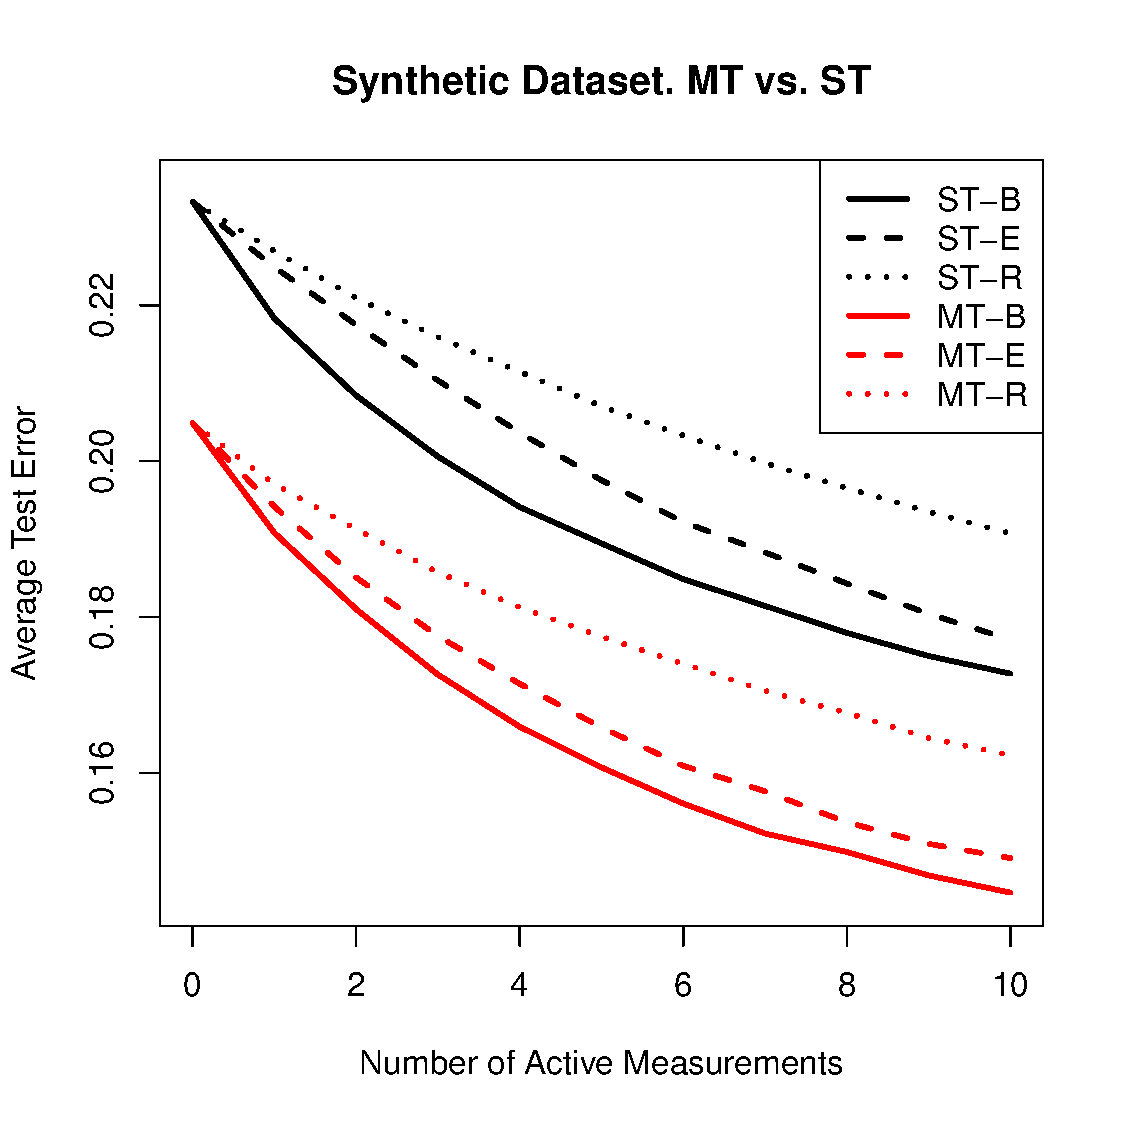
\includegraphics[scale = 0.3]{figs/plotsSyntheticData/plotSyntheticDatasetSTvsMT.pdf}
\hspace{-0.1cm}
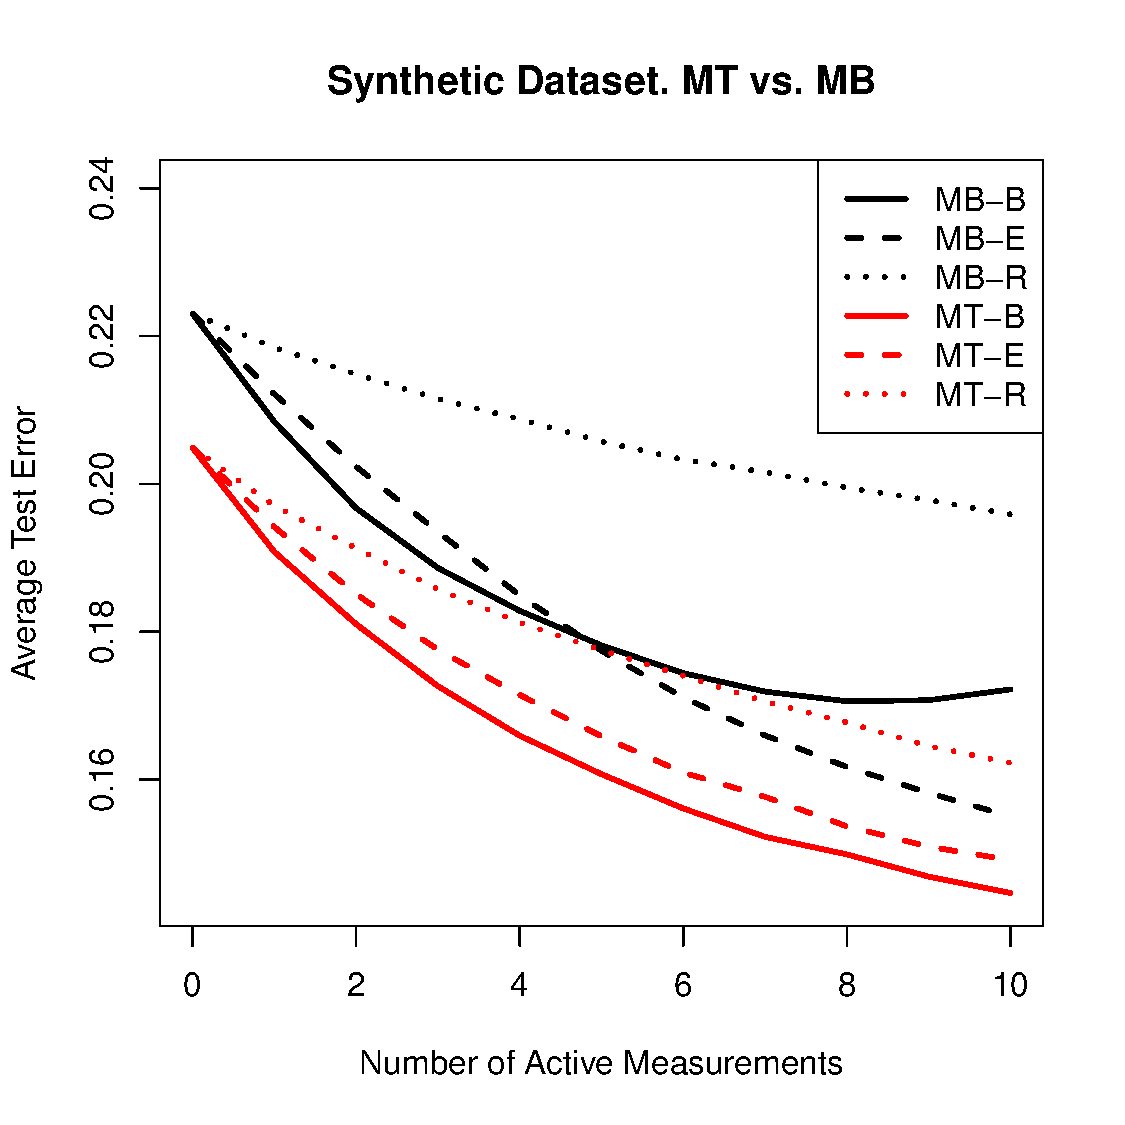
\includegraphics[scale = 0.3]{figs/plotsSyntheticData/plotSyntheticDatasetMBvsMT.pdf}
\hspace{-0.1cm}
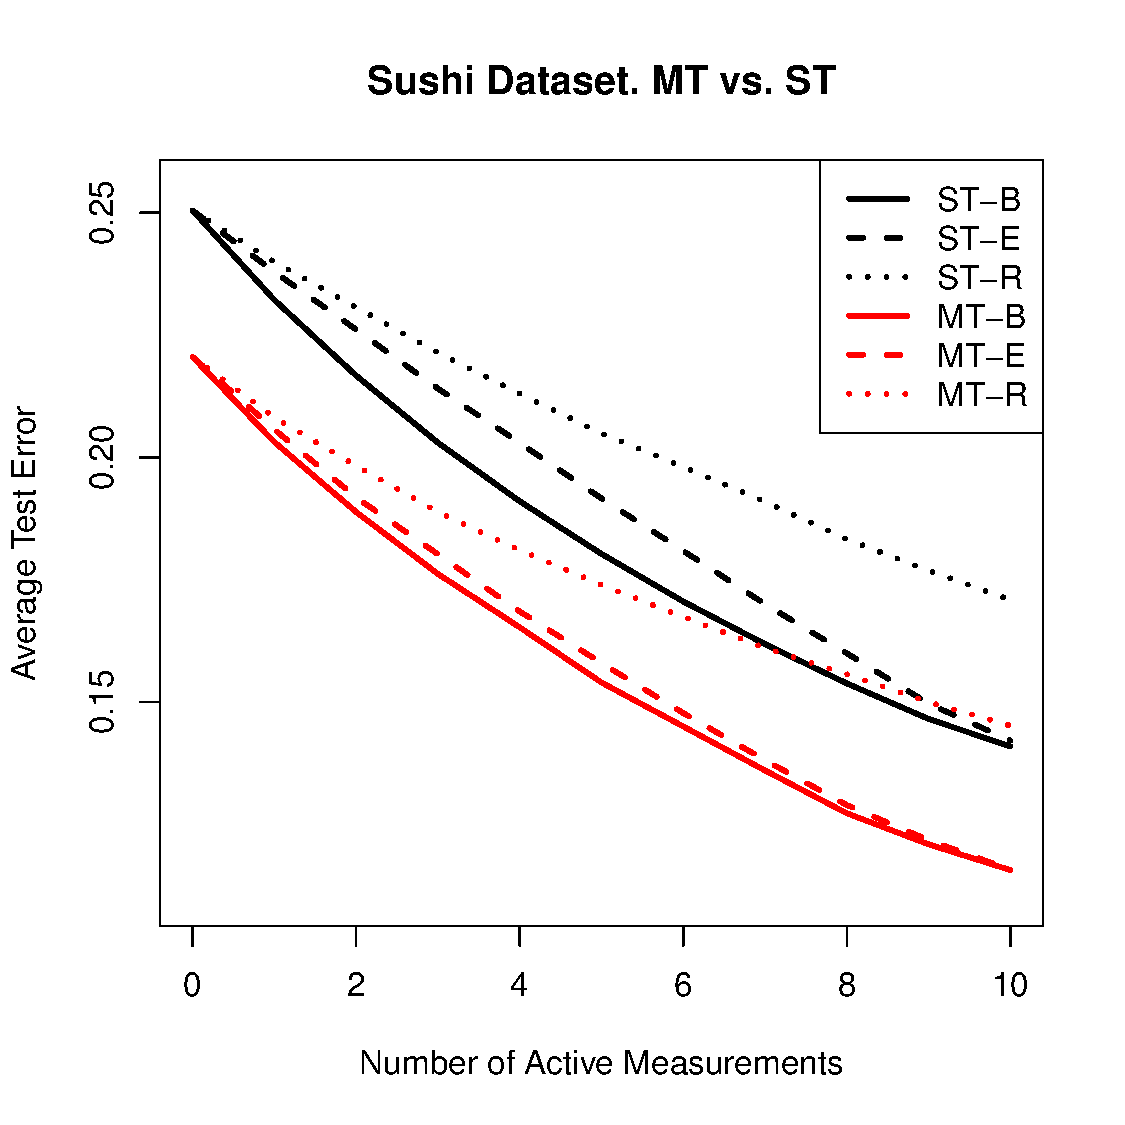
\includegraphics[scale = 0.3]{figs/plotsSushiData/plotSushiDatasetSTvsMT.pdf}
\hspace{-0.1cm}
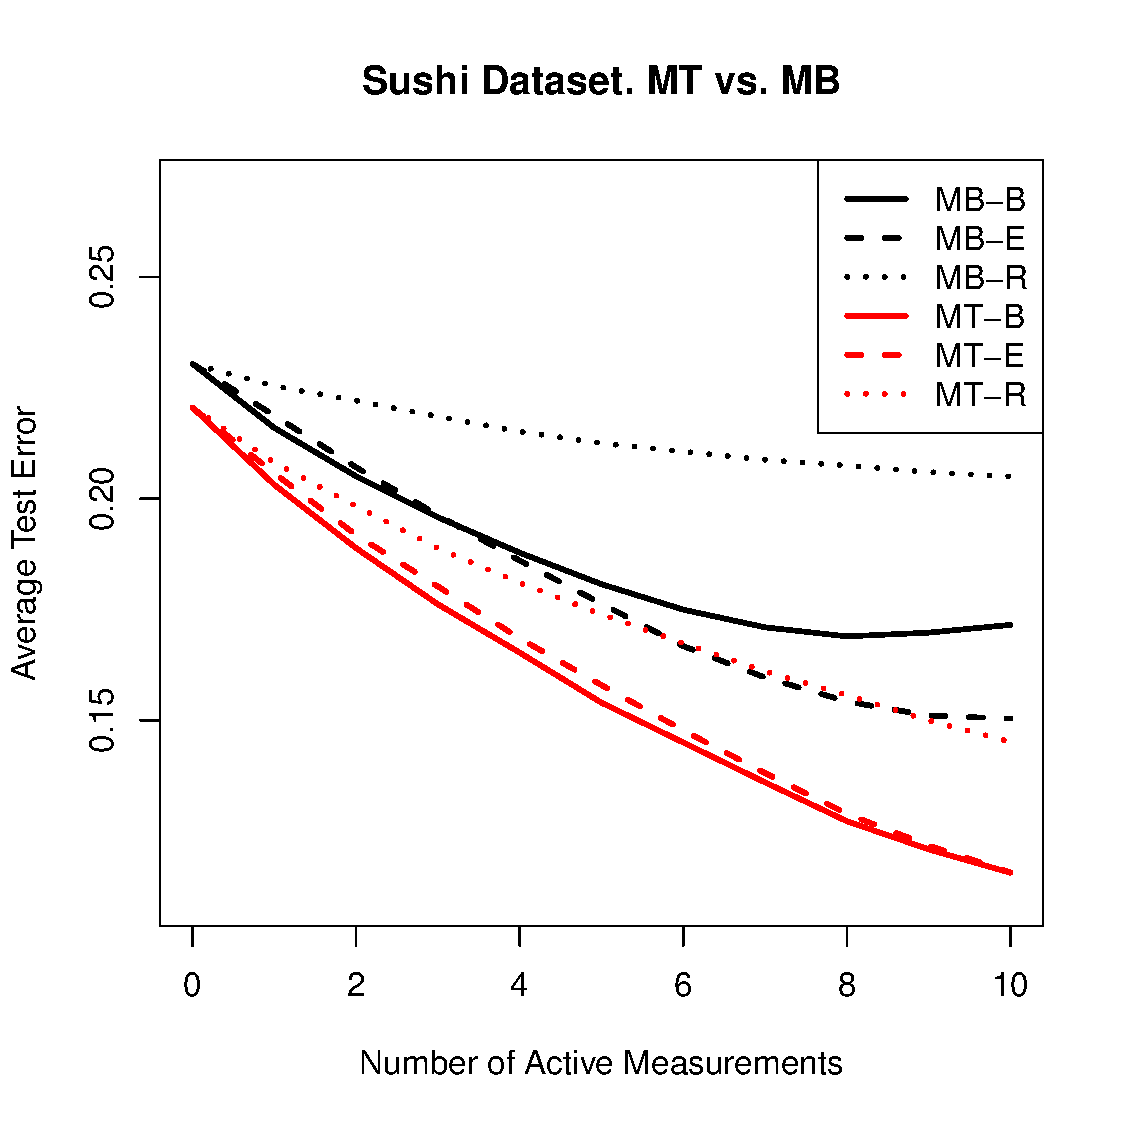
\includegraphics[scale = 0.3]{figs/plotsSushiData/plotSushiDatasetMBvsMT.pdf}
\caption{Top left, average test error as a function of the number of active measurements \DIFdelbeginFL \DIFdelFL{from the pool sets
}\DIFdelendFL for \DIFdelbeginFL \DIFdelFL{the proposed multi-task approach (}\DIFdelendFL MT \DIFdelbeginFL \DIFdelFL{) in the simulated data using BALD (MT-B), MES (MT-E) }\DIFdelendFL and \DIFdelbeginFL \DIFdelFL{a random method (MT-R)
for the selection of the most informative points }\DIFdelendFL \DIFaddbeginFL \DIFaddFL{ST }\DIFaddendFL in the \DIFdelbeginFL \DIFdelFL{pool set. This plot also shows the average test error on the }\DIFdelendFL simulated data\DIFdelbeginFL \DIFdelFL{for
the single task method (ST) using BALD (ST-B), MES (ST-E) and the random approach (ST-R)}\DIFdelendFL .
Top right, comparison on the simulated data \DIFdelbeginFL \DIFdelFL{of MT-B, MT-E }\DIFdelendFL \DIFaddbeginFL \DIFaddFL{between MT }\DIFaddendFL and \DIFdelbeginFL \DIFdelFL{MT-R with respect to the 
multi-task method given by }%DIFDELCMD < \citep{birlutiu2009} %%%
\DIFdelFL{(}\DIFdelendFL MB\DIFdelbeginFL \DIFdelFL{) using BALD (MB-B), MES (MB-E) and random (MB-R)
strategies for the selection of the most informative points}\DIFdelendFL .
Bottom left, \DIFdelbeginFL \DIFdelFL{comparison on the Sushi dataset }\DIFdelendFL \DIFaddbeginFL \DIFaddFL{average test error as a function }\DIFaddendFL of the \DIFdelbeginFL \DIFdelFL{results }\DIFdelendFL \DIFaddbeginFL \DIFaddFL{number }\DIFaddendFL of \DIFdelbeginFL \DIFdelFL{MT-B, MT-E and MT-R with respect to ST-B, ST-E }\DIFdelendFL \DIFaddbeginFL \DIFaddFL{active measurements for MT }\DIFaddendFL and \DIFdelbeginFL \DIFdelFL{ST-R}\DIFdelendFL \DIFaddbeginFL \DIFaddFL{ST in the Sushi dataset}\DIFaddendFL .
Bottom right, comparison on the Sushi dataset \DIFdelbeginFL \DIFdelFL{of the results of MT-B, MT-E and MT-R with respect to MB-B, MB-E }\DIFdelendFL \DIFaddbeginFL \DIFaddFL{between MT }\DIFaddendFL and \DIFdelbeginFL \DIFdelFL{MB-R}\DIFdelendFL \DIFaddbeginFL \DIFaddFL{MB}\DIFaddendFL .
}\label{fig:results}
\end{figure*}
\DIFaddbegin 

\DIFaddend \begin{table*}\centering
\caption{Results for the simulated data: test error $\pm 1\,\mathrm{s.d}$. Best performing algorithms highlighted in bold face.}
\label{tab:resultsSimulated}
\resizebox{\textwidth}{!}{
\begin{tabular}{c@{\hspace{0.2cm}}r@{$\pm$}l@{\hspace{0.2cm}}r@{$\pm$}l@{\hspace{0.2cm}}r@{$\pm$}l@{\hspace{0.2cm}}r@{$\pm$}l@{\hspace{0.2cm}}r@{$\pm$}l@{\hspace{0.2cm}}r@{$\pm$}l@{\hspace{0.2cm}}r@{$\pm$}l@{\hspace{0.2cm}}r@{$\pm$}l@{\hspace{0.2cm}}r@{$\pm$}l}
\hline
\bf{ $\bm n$}& \multicolumn{2}{c}{ \bf{ MT-B }}& \multicolumn{2}{c}{ \bf{ MT-E }}& \multicolumn{2}{c}{ \bf{ MT-R }}& \multicolumn{2}{c}{ \bf{ ST-B }}& \multicolumn{2}{c}{ \bf{ ST-E }}& \multicolumn{2}{c}{ \bf{ ST-R }}& \multicolumn{2}{c}{ \bf{ MB-B }}& \multicolumn{2}{c}{ \bf{ MB-E }}& \multicolumn{2}{c}{ \bf{ MB-R }}\\
\hline
0&\bf{20.49} & \bf{0.4}& \bf{20.49} & \bf{0.4}& \bf{20.49} & \bf{0.4}& 23.33 & 0.4& 23.33 & 0.4& 23.33 & 0.4& 22.30 & 0.5& 22.30 & 0.5& 22.30 & 0.5\\
3&\bf{17.26} & \bf{0.3}& 17.76 & 0.3& 18.57 & 0.3& 20.06 & 0.2& 21.03 & 0.2& 21.59 & 0.3& 18.86 & 0.3& 19.35 & 0.4& 21.15 & 0.4\\
5&\bf{16.07} & \bf{0.2}& 16.58 & 0.3& 17.75 & 0.3& 18.94 & 0.2& 19.76 & 0.3& 20.70 & 0.3& 17.81 & 0.4& 17.74 & 0.3& 20.57 & 0.4\\
7&\bf{15.22} & \bf{0.2}& 15.77 & 0.3& 17.05 & 0.3& 18.14 & 0.3& 18.83 & 0.3& 19.97 & 0.3& 17.19 & 0.4& 16.60 & 0.3& 20.16 & 0.5\\
10&\bf{14.47} & \bf{0.3}& 14.91 & 0.2& 16.23 & 0.2& 17.27 & 0.2& 17.71 & 0.2& 19.07 & 0.3& 17.22 & 0.4& 15.50 & 0.3& 19.59 & 0.5\\

\hline
\end{tabular}
}
\end{table*}


\DIFaddbegin 

\DIFaddend \begin{table*} \centering
\caption{Results for the Sushi dataset: test error $\pm 1\,\mathrm{s.d}$. Best performing algorithms highlighted in bold face.}
\label{tab:resultsSushi}
\resizebox{\textwidth}{!}{
\begin{tabular}{c@{\hspace{0.2cm}}r@{$\pm$}l@{\hspace{0.2cm}}r@{$\pm$}l@{\hspace{0.2cm}}r@{$\pm$}l@{\hspace{0.2cm}}r@{$\pm$}l@{\hspace{0.2cm}}r@{$\pm$}l@{\hspace{0.2cm}}r@{$\pm$}l@{\hspace{0.2cm}}r@{$\pm$}l@{\hspace{0.2cm}}r@{$\pm$}l@{\hspace{0.2cm}}r@{$\pm$}l}
\hline
\bf{ $\bm n$}& \multicolumn{2}{c}{ \bf{ MT-B }}& \multicolumn{2}{c}{ \bf{ MT-E }}& \multicolumn{2}{c}{ \bf{ MT-R }}& \multicolumn{2}{c}{ \bf{ ST-B }}& \multicolumn{2}{c}{ \bf{ ST-E }}& \multicolumn{2}{c}{ \bf{ ST-R }}& \multicolumn{2}{c}{ \bf{ MB-B }}& \multicolumn{2}{c}{ \bf{ MB-E }}& \multicolumn{2}{c}{ \bf{ MB-R }}\\
\hline
0&\bf{22.05} & \bf{0.4}& \bf{22.05} & \bf{0.4} & \bf{22.05} & \bf{0.4} & 25.05 & 0.4& 25.05 & 0.4& 25.05 & 0.4& 23.04 & 0.5& 23.04 & 0.5& 23.04 & 0.5\\
3&\bf{17.62} & \bf{0.4}& 18.02 & 0.3& 18.88 & 0.3& 20.30 & 0.4& 21.41 & 0.4& 22.14 & 0.3& 19.58 & 0.5& 19.63 & 0.4& 21.85 & 0.5\\
5&\bf{15.40} & \bf{0.3}& 15.79 & 0.2& 17.39 & 0.3& 18.03 & 0.4& 19.16 & 0.3& 20.49 & 0.4& 18.07 & 0.4& 17.63 & 0.4& 21.25 & 0.5\\
7&\bf{13.60} & \bf{0.3}& 13.81 & 0.2& 16.11 & 0.4& 16.18 & 0.3& 17.00 & 0.3& 19.09 & 0.3& 17.10 & 0.4& 15.97 & 0.4& 20.87 & 0.5\\
10&\bf{11.56} & \bf{0.2}& \bf{11.57} & \bf{0.2} & 14.52 & 0.3& 14.09 & 0.3& 14.21 & 0.3& 17.09 & 0.3& 17.15 & 0.4& 15.04 & 0.3& 20.50 & 0.4\\

\hline
\end{tabular}
}
\end{table*}


\DIFaddbegin \subsection{\DIFadd{Experiments with Real-world Data}}

\DIFaddend In the previous experiments with simulated data, MT \DIFdelbegin \DIFdel{obtained the best performance. This was }\DIFdelend \DIFaddbegin \DIFadd{obtains the best results. This is }\DIFaddend expected because the data \DIFdelbegin \DIFdel{were }\DIFdelend \DIFaddbegin \DIFadd{are }\DIFaddend actually sampled
from the probabilistic model assumed by this method. To obtain more representative results, we perform another series of experiments
\DIFaddbegin \DIFadd{with }\DIFaddend the real-world Sushi dataset \citep{kamishima2003}\DIFdelbegin \DIFdel{, see Fig.}%DIFDELCMD < \,%%%
\DIFdel{\ref{fig:results}, bottom plots}\DIFdelend .
This dataset contains complete rankings given by 5000 users over a total of $I = 10$ different types of sushi,
where each sushi is represented by a set of features including style, major group, minor group, heaviness, consumption
frequency, normalized price and sell frequency. The first three featuers \DIFaddbegin \DIFadd{in the dataset }\DIFaddend are categorical. We encoded \DIFdelbegin \DIFdel{these
features }\DIFdelend \DIFaddbegin \DIFadd{them
}\DIFaddend using dummy binary variables\DIFdelbegin %DIFDELCMD < \citep{bonilla2010}%%%
\DIFdelend .
Each sushi is represented by a 15-dimensional feature vector. We \DIFdelbegin \DIFdel{reduce }\DIFdelend \DIFaddbegin \DIFadd{reduced }\DIFaddend the size of the dataset by
randomly sub-sampling $U=1000$ users. For each of these users, the available preference data are 
\DIFdelbegin \DIFdel{now }\DIFdelend randomly split into training, pool and test sets with 10, 20 and 25 elements, respectively.
\DIFdelbegin \DIFdel{The configuration for the different methods is also the same as before except that we now }\DIFdelend \DIFaddbegin \DIFadd{In this case we }\DIFaddend use a total of $D=50$ latent functions in MT. 
The results obtained by this method are not \DIFdelbegin \DIFdel{very }\DIFdelend sensitive to the exact value of this parameter as long as it is not excessively low.
Finally, we always standardize the item features so that they have zero mean and unit standard deviation in the training set and 
set the length-scale parameter \DIFdelbegin \DIFdel{($\sigma$) of the preference }\DIFdelend \DIFaddbegin \DIFadd{of the squared exponential }\DIFaddend kernel to one. 
In practice, the kernel parameter should be learned to obtain the best possible performance.
This can be done in \DIFdelbegin \DIFdel{the proposed multi-task approach (MT ) and in the single task method (ST) }\DIFdelend \DIFaddbegin \DIFadd{MT }\DIFaddend by searching for the parameter value that
maximizes the EP approximation of the model evidence\DIFaddbegin \DIFadd{, as illustrated in the suplementary material}\DIFaddend .
The cost of this search is too expensive for the proposed experimental protocol.
Nevertheless, we expect that using the same value for the kernel parameter in all
methods leads to an unbiased comparison of performances.
\DIFdelbegin \DIFdel{In the supplementary material we present an experiment that shows that $\sigma=1$ yields the highest model evidence for MT, this result is supported by cross-validation.
}\DIFdelend 

\DIFdelbegin \DIFdel{The MT techniques are }\DIFdelend \DIFaddbegin \DIFadd{The bottom plots in Figure \ref{fig:results} show the results of MT, ST and MB in the Sushi dataset.
MT is }\DIFaddend markedly superior to \DIFdelbegin \DIFdel{the corresponding }\DIFdelend ST and MB\DIFdelbegin \DIFdel{methods}\DIFdelend . The differences between the BALD and MES alternatives are also significant, with BALD outperforming MES in general.
However, for more than 5 active measurements \DIFdelbegin \DIFdel{the errors of }\DIFdelend MT-B and ST-B seem to converge to \DIFdelbegin \DIFdel{the errors of }\DIFdelend MT-E and ST-E, respectively.
This result is likely to have its origin in the reduced size of the pool set\DIFaddbegin \DIFadd{, }\DIFaddend which only contains 20 points in this case.
Furthermore\DIFaddbegin \DIFadd{, }\DIFaddend if subjects exhibit low noise in their preferences \DIFdelbegin \DIFdel{judgements }\DIFdelend then MES approaches BALD because the second term in Equation \eqref{eqn:BALD} becomes small.
We also note \DIFdelbegin \DIFdel{pathological performance }\DIFdelend \DIFaddbegin \DIFadd{a pathological behaviour }\DIFaddend of MB-B \DIFdelbegin \DIFdel{, this is because of the unimodal a prior over preference functionsused in MB which is a poor model
for these data. When using BALD this misspecified model is
learnt rapidly and performance decreases after eight samples. Table \ref{tab:resultsSushi} }\DIFdelend \DIFaddbegin \DIFadd{as more data points are added to the training set.
Similar patterns can be observed for the simulated data.
This result is probably due to fact that MB assumes a common unimodal prior for preference functions. An assumption which is
unlikely to be true in practice. Finally, Table \ref{tab:resultsSimulated} }\DIFaddend provides detailed results for \DIFdelbegin \DIFdel{the sushi data.
 }%DIFDELCMD < 

%DIFDELCMD <  %%%
\DIFdelend \DIFaddbegin \DIFadd{each method on the Sushi dataset.
 }\DIFaddend